\documentclass[__main__.tex]{subfiles}

\begin{document}
\paragraph{Э-21}
Сила Ампера. Магнитное поле прямого постоянного тока. Сила взаимодействия двух постоянных токов.\\

В ходе экспериметов Ампер установил, что сила, с которой магнитное поле действует на проводник зависит от: 
\begin{enumerate}
	\item длины проводника $l$
	\item силы тока $I$
	\item величины магнитного поля $\vec B$
	\item угла между проводником и $\vec B$
\end{enumerate}
\begin{gather*}
	d\vec F_A = I \left[ d\vec l\times\vec B\right],
\end{gather*}
где $d\vec F_A$ - элементарная сила Ампера, действующая на проводник $dl$ с током $I$, находящимся в магнитном поле $\vec B$.
\\
Для определения магнитного поля, нужно познакомиться с законом Био-Савара-Лапласа, вывод которого здесь приведён не будет:
\begin{gather*}
	d\vec B = \frac{\mu_0}{4\pi}\frac{I\cdot\left[d\vec l\times\vec r\right]}{r^3},
\end{gather*}
где $d\vec B$ - вектор магнитной индукции, создаваемый элементом $d\vec l$, а $\vec r$ - вектор от элемента проводника до точки наблюдения поля.
\begin{figure}[h]
	\centering
	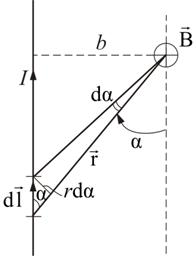
\includegraphics[width=.23\linewidth]{e-21}
\end{figure}
Далее по рисунку сверху:
\begin{gather*}
	r = \frac{b}{\sin\alpha};\quad
	dl = \frac{r\cdot d\alpha}{\sin\alpha} = \frac{b\cdot d\alpha}{\sin^2\alpha}\Rightarrow\\
	dB = \frac{\mu_0}{4\pi}\frac{I}{b}\sin\alpha d\alpha\Rightarrow B = \int_{0}^{\pi}dB = \frac{\mu_0}{4\pi}\frac{2I}{b}.
\end{gather*}
\\
Представим, что в вакууме на расстоянии $r$ друг от друга расположены 2 бесконечно длинных тонких проводника, в которых в одном направлении текут токи $I_1$ и $I_2$. По БСЛ 1-й проводник на расстоянии $r$  создаёт поле:
\begin{gather*}
	B_1(r) = \frac{\mu_0}{4\pi}\frac{2I_1}{r}.
\end{gather*}
Теперь из Ампера найдём силу, с которой 1-й проводник действует на 2-й:
\begin{gather*}
	d\vec F_{1-2} = I_2\cdot d\vec l\times\vec B_1(r)\Longrightarrow\\
	dF_{1-2} = \frac{\mu_0}{4\pi}\frac{2I_1I_2}{r}dl\Longrightarrow\\
	F_{1-2} = \frac{\mu_0}{4\pi}\frac{2I_1I_2}{r}
\end{gather*}
\end{document}